\documentclass [titlepage,12pt,letter] {article}
\pagestyle{myheadings}


\usepackage{graphicx} 
\usepackage{epsfig}
\usepackage{subfigure}
\usepackage{fancyhdr}
\usepackage{url} 
\pagestyle{fancy}


\fancyhead{}
\fancyfoot{}
			
\lhead{CSC349A Lecture Notes}
\rhead{Little, Rich}


\setcounter{page}{1}
\cfoot{\thepage}




\begin{document} 


These are the lecture notes for CSC349A Numerical Analysis taught by
Rich Little. They roughly correspond to
the material covered in each lecture in the classroom but the actual
classroom presentation might deviate significantly from them depending
on the flow of the course delivery. They are provide as a reference to
the instructor as well as supporting material for students who miss
the lectures. They are simply notes to support the lecture so the text
is not detailed and they are not thoroughly checked. Use at your own
risk. They are complimentary to the handouts.

\section{Overview} 

In this lecture we reviewed the Newton/Raphson method
for root finding as an example of an open method (i.e requires only an
initial estimate of the root) in contrast to bracketing methods like
Bisection which require an interval to bound the root. This included two derivations 
of the algorithm, an example of the algorithm and analysis of the error convergence.
The exact details are provided below.


\section{Newton-Raphson} 

\subsection{Geometric derivation}

The real roots of a function $f(x)$ occur when the graph of the
function intersects with the x-axis. The main idea behind the
Newton/Raphson method for root finding is given an initial
approximation $x_0$ to a zero of $f(x)$ to approximate the graph of $f(x)$
at $x_0$ by the {\bf tangent line} - essentially linearizing the function in
that area. Figure 1 shows this visually. 


\begin{figure}[ht]
  \centering
  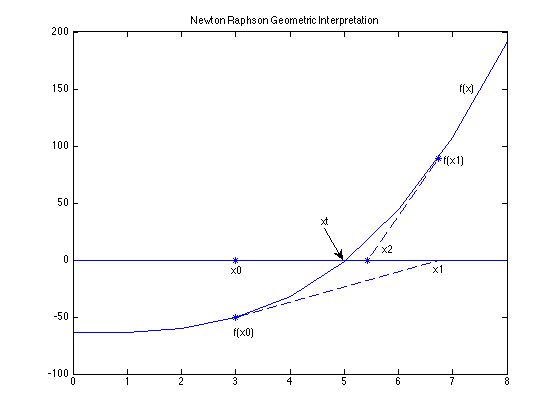
\includegraphics[scale=0.75]{newton}
  \caption{Geometric interpetation of the Newton Raphson method for
    root finding.}
  \label{fig:newton}
\end{figure}

\noindent 
Let $x_1$, the intersection of the tangent line with the $x$-axis, be
the next approximation to $x_t$. The slope of the tangent line is: 
\begin{equation}
f'(x_0)=\frac{f(x_0)-0}{x_0-x_1} 
\end{equation} 
\noindent Thus the tangent line intersects the $x$-axis when
\begin{equation} 
f'(x_0)(x_0-x_1) = f(x_0)
\end{equation} 
\noindent 
so the next estimate $x_1$ can be calculated as: 
\begin{equation} 
x_{1} = x_{0} - \frac{f(x_0)}{f'(x_0)}
\end{equation}

The process can be repeated starting from the new root estimate $x_1$
with the following equation. 

\begin{equation} 
x_2 = x_1 - \frac{f(x_1)}{f'(x_1)}
\end{equation}

In general, we calculate a new root estimate $x_{i+1}$ from the previous estimate
$x_i$ with the following equation. 

\begin{equation} 
x_{i+1} = x_i - \frac{f(x_i)}{f'(x_i)}
\end{equation} 

\subsection{Example of Newton-Raphson Method} 

Estimate the root of $f(x) = e^{-x} -x$ employing an initial guess of
$x_0 = 0$. 
Note that $x_t$ = 0.56714329... is the actual root. Also, $f'(x) = -e^{-x} - 1$ and thus

\begin{equation}
x_{i+1} = x_i - \frac{e^{-x_i} - x_i}{-e^{-x_i}-1}
\end{equation}

\noindent
This iterative equation can be applied to compute: 

\begin{table}[h]
\begin{tabular}{c|c|c} 
$i$ & $x_i$ & $\varepsilon_t(\%)$ \\ 
\hline 
$0$ & $0$ & $100$ \\
$1$ & $0.5$ & $11.8$ \\ 
$2$ & $0.566311003$ & $0.147$ \\
$3$ & $0.567143165$ & $0.0000220$ \\ 
$4$ & $0.567143290$ & $<10^{-8}$ \\  
\hline
\end{tabular} 
\end{table} 
\noindent 
Notice that the approach rapidly converges on the true root much faster than 
it would using {\it Bisection}. 

\section{Newton method convergence}

Consider the Taylor theorem for $f(x)$ with $n=1$ expanded about
$x_i$ (i.e $a = x_i$): 

\begin{equation} 
f(x) = f(x_i) + (x-x_i) f'(x_i) + \frac{f''(\xi)}{2}(x-x_i)^2
\end{equation}
\noindent 
for some value $\xi$ between $x$ and $x_i$. 

The derivation of the Newton/Raphson method gives insight into how
fast Newton's method converges:
\\
First we evaluate the Taylor Theorem at $x=x_t$, an exact zero: 

\begin{equation} 
0 = f(x_t) = f(x_i) + (x_t-x_i)f'(x_i) + \frac{(x_t-x_i)^2}{2}f''(\xi)
\end{equation} 

Newton's method $x_{i+1} = x_{i} - \frac{f(x_i)}{f'(x_i)}$ can be rewritten as: 
\begin{equation} 
0 = f(x_i) + (x_{i+1} -x_{i}) f'(x_{i})
\end{equation} 
\noindent 
If we subtract the last two equations then we get: 

\begin{equation} 
0 = (x_t -x_{i+1}) f'(x_i) + \frac{(x_t - x_i)^2}{2}f''(\xi)
\end{equation} 
\noindent or if we let $E_{i+1} = x_t - x_{i+1}$ and $E_i = x_t - x_{i}$ denote the error in $x_{i+1}, x_i$ then we have: 
\begin{equation} 
0 = E_{i+1} f'(x_i) + \frac{E_i^2}{2} f''(\xi) 
\end{equation} 
\noindent 
Thus: 
\begin{equation} 
\frac{E_{i+1}}{E_i^2} = \frac{-f''(\xi)}{2f'(x_{i})} 
\end{equation} 
\noindent 
which relates $E_{i+1}$ to $E_i$. 
\noindent 
\\
\subsection{Definition (not in textbook)}  
If a sequence ${x_0, x_1, x_2, x_3, \dots }$ converges to $x_t$ that is 
$\lim_{i \rightarrow \infty}x_i = x_t$ and $E_i = x_t - x_i$, then the order of converge of the sequence is $\alpha$ if there are constants $\lambda > 0$ and $\alpha \geq 1$ such that: 
\begin{equation} 
\lim_{i \rightarrow \infty} \frac{|E_{i+1}|}{|E_i|^{\alpha}} = \lambda 
\end{equation} 

In general, $\lambda$ and $\alpha$ depend on the algorithm used to compute ${x_i}$, on $f(x)$, and on the multiplicity of the zero $x_t$. 

{\bf Most common case:} 
\\ 
$\alpha = 1$ linear convergence \\ 
For large $i$, $|E_{i+1}| \approx \lambda |E_i|$ \\ 


In this case, successive errors decrease approximately by a constant amount: 
\begin{eqnarray*} 
|E_{i+1}| &\approx & \lambda |E_i| \\ 
|E_{i+2}| &\approx &  \lambda |E_{i+1}| \approx \lambda^2 |E_i|\\ 
|E_{i+3}| & \approx &  \lambda |E_{i+2}| \approx \lambda^3 |E_i|\\ 
\mbox{etc} \\ 
\end{eqnarray*} 

Errors $|E_{i+1}| \rightarrow 0$, that is $\lim_{i \rightarrow \infty}
x_i = x_t$ only if $0 < \lambda < 1$.

For $\alpha = 2$ we have quadratic convergence. For large $i$, $|E_{i+1}| \approx \lambda |E_i|^2$ 
\\
Meaning: after some error $|E_i| < 1$, convergence is rapid as the number of correct significant digits approximately doubles with each iteration e.g if 
$|E_i| = 10^{-t}$, then $|E_{i+1}| \approx \lambda 10^{-2t}$. 

For Newton's method above: 
\[ 
\frac{E_{i+1}}{E_{i}^2} = \frac{-f''(\xi)}{2f'(x_i)} 
\] 
\noindent for some $\xi$ between $x_i$ and $x_{i+1}$. 

\[
\lim_{i \rightarrow \infty} \frac{|E_{i+1}|}{|E_i|^2} = \lim_{i \rightarrow \infty} 
\frac{|f''(\xi)|}{2|f'(x_i)|} = \frac{|f''(x_t)|}{2|f'(x_t)|}
\]
\noindent 
which is a constant $\lambda$ provided that $f'(x_t) \neq 0$. 
\\

\section{Implementation}

The algorithm for Newton's method can be written in pseudocode as
follows: 

\begin{tabbing}
  xxx \= xxx \= xxx \= xxx \kill
\> \textbf{function} root = Newton( $x_0$, $\varepsilon$, \texttt{imax} ) \\
\> $i \leftarrow 1$ \\
\> output heading \\
\> \textbf{while} $i \le $ \texttt{imax} \\
\> \> $root \leftarrow x_0 - f(x_0)/f'(x_0)$ \\
\> \> output $i$, root \\
\> \> \textbf{if} $|1-x_0/root| < \varepsilon$ \\
\> \> \> exit \\
\> \> \textbf{end if} \\
\> \> $i \leftarrow i + 1$ \\
\> \> $x_0 \leftarrow root$ \\
\> \textbf{end while} \\
\> output ``failed to converge"
\end{tabbing}

\noindent 
Note that in general, using $|f(root)| < \varepsilon$ is not a suitable
test for convergence (instead of testing approximation error). The
reason is that $|f(root)| < \varepsilon$ does not imply that the value
{\it root} is within distance of $\varepsilon$ of an exact root $x_t$. 



\section{Quadratic convergence of Newton's method} 

{\bf Theorem}: If Newton's method is applied to $f(x) = 0$ producing 
a sequence $x_i$ that converges to a root $x_t$, and if $f'(x_t) \neq 0$, then 
then order of convergence is $2$. 

If $f'(x_t) = 0$ and Newton's method convergences to a root $x_t$, then we will see later that the order of convergence is NOT quadratic. \\ 

\medskip 
\noindent 
{\bf Example 1} An illustration of the quadratic convergence of Newton's method. Here $f(x) = cos(x) -x$. This was computed in MATLAB, so at most 16 correct digits are possible. The bold digits are all correct. 


\begin{table}[h] 
\begin{tabular}{c|l|c}
$i$ & $x_i$ & no. of correct digits \\ 
\hline
0   & $\frac{\pi}{4} = 0.{\bf 7}85398$ & 1 \\ 
1   & 0.{\bf 739}5361 & 3 \\ 
2   & 0.{\bf 7390851}78 & 7 \\ 
3   & 0.{\bf 73908513321516}10 & 14 \\ 
4   & 0.{\bf 7390851332151606}  & 16 \\ 
\end{tabular} 
\end{table}  


\medskip 
\noindent 
{\bf Example 2}. The following illustrates the possible effect of a poor initial approximation with Newton's method, yet the eventual characteristic quadratic convergence. Here Newton's method is used to compute a root of $x^3 + 4 x^2 -10 = 0$ with $p_0 = -100$. Partial results are as follows. 

\begin{table}[h]
\begin{tabular}{l|c}
$p_0 = -100$ &  \\ 
$p_1 = -67.12$ &  \\ 
$p_2 = -45.21$ &  \\ 
$\dots$ & $\dots$ \\ 
$p_{14} = -2.54$ &  \\ 
$p_{15} = -3.14$ &  \\ 
$p_{16} = -2.80$ &  \\ 
$\dots$ & $\dots$ \\ 
$p_{21} = 1.9405$ &  no. of correct digits \\ 
$p_{22} = {\bf 1}.4793$ &  $1$ \\ 
$p_{23} = {\bf 1.3}711$ &  $2$ \\ 
$p_{24} = {\bf 1.365}25$ &  $4$ \\ 
$p_{25} = {\bf 1.365230001}1$  &  $9$ \\ 
\end{tabular} 
\end{table} 

I ran this example with a Newton function of my own devising that also recorded $|E_{i+1}|$/$|E_i|$ at each step to give you an idea of how this example is converging. This value is given in the third column of the output:

\begin{verbatim}
>> Newton_wCR(-100,10^(-8),1000,@Ex2,@Ex2Prime,xt)
 iteration approximation 
      0 -100.0000000000000000 
      1 -67.1229452054794540 0.6756574735718571 
      2 -45.2106915629508280 0.6800578556444912 
      3 -30.6110303374327980 0.6865405829580693 
      4 -20.8903135326827250 0.6960020747237687 
      5 -14.4275998450253840 0.7096133071622610 
      6 -10.1439728120448680 0.7287612751243944 
      7 -7.3216506641581773 0.7547769215046272 
      8 -5.4823476696099007 0.7882665754466991 
      9 -4.3043281697322326 0.8279655150465651 
     10 -3.5648242613362786 0.8695658665971102 
     11 -3.0994781840095929 0.9056103540867716 
     12 -2.7643039450246527 0.9249280749908025 
     13 -2.0756744750764016 0.8332428121722965 
     14 -2.5401125042410282 1.1349755654997482 
     15 -3.1421077624340263 1.1541465967380635 
     16 -2.8006794352317459 0.9242505567184756 
     17 -2.2742377750642446 0.8736310362342069 
     18 -2.6754008707963317 1.1102257580083743 
     19 4.7255390285480541 0.8316297903540348 
     20 2.9616670020385882 0.4750863630203516 
     21 1.9405440180104074 0.3603737627577821 
     22 1.4793327062840065 0.1983311582167616 
     23 1.3711198338928769 0.0516185931343018 
     24 1.3652469470192556 0.0028750630379588 
     25 1.3652300135546727 0.0000083015856297 
     26 1.3652300134140969 0.0000000000000000 

ans =

    1.3652
\end{verbatim}

\noindent
Notice how the convergence rate actually looks linear for the first 20 iterations in this example. This reitereates that the quadratic
convergence only occurs once we get close to the actual root. If your first approximation is far away then the convergence is not 
entirely quadratic.

Your text illustrates four cases where Newton has poor convergence or divergence. I have inserted it here as well.

\begin{figure}[ht]
  \centering
  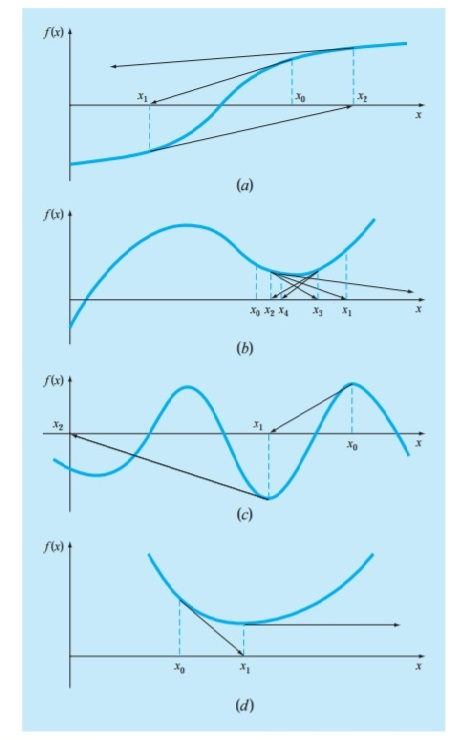
\includegraphics[scale=1]{BadNewton}
%   \caption{Geometric interpetation of the Newton Raphson method}
  \label{fig:BadNewton}
\end{figure}


\noindent 
{\bf Theorem} Suppose that $f(x),f'(x)$ and $f''(x)$ all exist and are continuous on some interval $[a,b]$, that $x_t \in [a,b]$ is a root of $f(x) = 0$, and that $f'(x_t) \neq 0$. Then there exists a value $\delta > 0$, such that Newton's method converges for all initial approximations $x_0 \in [x_t - \delta, x_t + \delta]$. 

{\bf Note} that in general there is no way to determine such a value $\delta$. This theorem only says that for all such functions $f(x)$, such a value $\delta$ exists. Even if the value of $\delta$ is extremely small, there is an interval of values around the root $x_t$ such that if $x_0$ (the initial approximation) lies in this interval, then Newton's method will converge. 

Thus the interpretation of the above theorem is that Newton's method always converges if the initial approximation $x_0$ is sufficiently close to the root $x_t$. 

In the process of writing these notes I used MATLAB to create the
figure illustrating the geometric interpretation of the Newton/Raphson
method. For those of you who are curious here is the relevant code. It
is quickly written and could easily be cleaned up and some comments
added. I also used the ability to add text boxes and text arrow boxes
in the Figure window.

\begin{verbatim} 
x = 0:8;
fx = 0.5 * x.^3 -64;
plot(x,fx);
hold;
x0=3;
fx0 = 0.5 * x0.^3-64;
x1 = x0 - (0.5 * x0.^3-64)/(1.5 * x0.^2);
plot([x0,x1],[fx0,0],'--');
plot(x, zeros(size(x)));
plot(x0,0,'*');
plot(x0,fx0, '*');
x2 = x1 - (0.5 * x1.^3-64)/(1.5 * x1^2);
fx1 = 0.5 * x1.^3-64;
plot(x2,0,'*');
plot([x1,x2],[fx1,0],'--');
plot(x1,fx1,'*')
\end{verbatim} 

\section*{Appendix} 

Sir Isaac Newton (1642-1726) - During much of 1665-1666, immediately after Newton had earned
his degree from Trinity College, Cambridge, the college was closed due to the black plague. Newton
went home to live and think during those two years. The result was the most productive period of
mathematical discovery ever reported. During that time he made four of his greatest mathematical
discoveries: (1) the binomial theorem, (2) calculus, (3) the law of gravity, and (4) the colour spectrum.

While Newton needs no introduction I was always curious about who
Raphson was. I was under the mistaken impression that he was some
mathematician in the 20th century who ``re-discovered'' Newton's
method. It turns out that's not the case. He was relatively a
contemporary of Newton and a member of the famous Royal Philosophical
Society. He supported Newton's claim to the invention of calculus in the
famous debate between Newton and Leibnitz about who invented
first. One tidbit of minor information that I found particularly
interesting was that he also was known for translating one of Newton's
books into English. It is easy to forget that at the time all
scientific communication was still conducted in Latin even though
Latin was a language that had not been spoken for centuries.






\bibliographystyle{IEEEbib} 
\bibliography{csc349a} 

\end{document} 











